\documentclass[preprint,12pt,authoryear]{elsarticle}
\makeatletter
\def\ps@pprintTitle{%
	\let\@oddhead\@empty
	\let\@evenhead\@empty
	\def\@oddfoot{\centerline{\thepage}}%
	\let\@evenfoot\@oddfoot}
\makeatother
\usepackage{booktabs}
\usepackage{subfigure, epsfig, epstopdf}
\usepackage{graphicx}
\usepackage{amsmath}
\usepackage{mathrsfs}
\usepackage{amssymb}
\usepackage{multirow, multicol}
\usepackage{color}
\usepackage{soul}
\usepackage{setspace}
\usepackage[left=0.8in,top=1in,right=0.8in,bottom=1in, nohead]{geometry}
\usepackage[colorlinks=true,backref=true,hyperindex,citecolor=blue,linkcolor=blue]{hyperref}
\usepackage{natbib}
\usepackage{tabularx}
\usepackage{colortbl}
\usepackage{titlesec}
\usepackage{enumerate}
\usepackage{amsfonts}
\usepackage{threeparttable}
\usepackage{float}
\usepackage{url}
\usepackage{hyperref}
\usepackage[titletoc,title]{appendix}
\usepackage{booktabs}
\usepackage{csvsimple}
%times new roman
%\usepackage[T1]{fontenc}
%\usepackage{newtxmath,newtxtext}
%helvetica
%\usepackage[scaled]{helvet}
%\renewcommand\familydefault{\sfdefault} 
%\usepackage[T1]{fontenc}

\titleformat{\paragraph}[block]{\normalsize\bfseries}{\theparagraph}{1em}{}

\bibpunct{(}{)}{;}{a}{,}{,}


\newtheorem{theorem}{Theorem}
\newtheorem{lemma}{Lemma}
\newtheorem{proposition}{Proposition}
\newtheorem{corollary}[theorem]{Corollary}
\newtheorem{assumption}{Assumption}

\newenvironment{proof}{\paragraph{Proof.}}{\hfill$\square$}
\newenvironment{definition}[1][Definition]{\begin{trivlist}
		\item[\hskip \labelsep {\bfseries #1}]}{\end{trivlist}}
\newenvironment{example}[1][Example]{\begin{trivlist}
		\item[\hskip \labelsep {\bfseries #1}]}{\end{trivlist}}
\newenvironment{remark}[1][Remark]{\begin{trivlist}
		\item[\hskip \labelsep {\bfseries #1}]}{\end{trivlist}}
\newenvironment{mydescription}{\begin{description}
		\setlength{\itemsep}{0pt}\setlength{\parskip}{0pt}\setlength{\parsep}{0pt}}{\end{description}} 

\newcommand{\bI}{\mathcal I}
\newcommand{\bN}{\mathcal N}
\newcommand{\bE}{\mathbb E}
\newcommand{\bR}{\mathfrak R}
\newcommand{\bQ}{\mathbb Q}
\newcommand{\bF}{\mathbb F}
\newcommand{\bP}{\mathbb P}
\newcommand{\by}{\mathbf y}
\newcommand{\bX}{\mathbf X}
\newcommand{\bT}{\mathbf T}
\newcommand{\bD}{\mathbf D}
\newcommand{\bt}{\mathbf t}
\newcommand{\bx}{\mathbf x}
\newcommand{\bs}{\mathbf s}
\newcommand{\bU}{\mathcal U}
\newcommand{\bW}{\mathcal W}
\newcommand{\pr}{\textup{Pr}}


\newcommand{\mb}[1]{\mbox{\boldmath \ensuremath{#1}}}
\renewcommand{\vec}[1]{\boldsymbol{#1}} 
\newcommand{\vectilde}[1]{\tilde{\boldsymbol{\boldsymbol{#1}}}}
\newcommand{\tildevarepsilon}{\tilde{\varepsilon}}
\newcommand{\vecvarepsilon}{\vec{\varepsilon}}
\newcommand{\vectildevarepsilon}{\tilde{\vec{\varepsilon}}}
\newcommand{\vectau}{\vec{\tau}}
\newcommand{\vecalpha}{\vec{\alpha}}
\doublespacing
\graphicspath{{imgs/}} 


\begin{document}
\setlength{\abovedisplayskip}{3pt}
\setlength{\belowdisplayskip}{3pt}

\begin{titlepage}
    \begin{center}
        \vspace*{1cm}
        
        \Huge
	 \textbf{Optimal design of decentralized constructed wetland treatment system under uncertainties}\\        
	 \noindent\makebox[\linewidth]{\rule{0.7\paperwidth}{0.4pt}}
        \vspace{0.5cm}
        \LARGE
        IE4100 Progress Report
        
        \vspace{1.5cm}
        
        Yeow Li Teng Cheryl\\
	  A0116781A\\
	  Mentor: A/P Ng Tsan Sheng, Adam
        
        \vfill
        
        \vspace{0.8cm}
        
%        \includegraphics[width=0.4\textwidth]{university}
        
        \Large
        Department of Industrial \& Systems Engineering\\
        National University of Singapore\\
%        Country\\
%        Date
        
    \end{center}
\end{titlepage}

%\begin{frontmatter}
	

	
%	  \title{\textbf{Optimal design of decentralized constructed wetland treatment system under uncertainties}}

%\begin{abstract}

%\end{abstract}

%\begin{keyword}

%\end{keyword}
%\end{frontmatter}



 
\section{Introduction}
Constructed wetlands is a wastewater treatment method that makes use of vegetation to treat wastewater. This treatment method requires very little energy and require significantly less human resources as it operates passively, unlike technology in centralized wastewater systems.

Decentralized wastewater management systems such as constructed wetlands are increasingly gaining traction as the costs of construction become comparable to centralized wastewater management systems. This is because of the many advantages decentralized systems give over centralized ones. For one, a decentralized system has more treatment sites, which reduces the impact of the failure of a treatment site. If a centralized treatment plant were to fail, the wastewater collected will accumulate and there is no backup plant available to treat the water. On the other hand, if one treatment site of a decentralized system fails, the wastewater may be rerouted to other sites temporarily, ensuring that the system does not come to a standstill. 

While constructed wetlands can essentially be implemented wherever there is space, the maximum effectiveness of using this decentralized wastewater treatment system is only achieved when it is located at an optimal distance to the areas which it serves. The performance of constructed wetlands also depends on whether the size is sufficient to handle the projected wastewater flow rate from the area. In addition, the components of wastewater is easily affected by the source and weather. Due to this natural variation, the pollutant composition in wastewater is not deterministic. The ideal configuration (location and size) of treatment sites from a deterministic optimization model may not be feasible under such uncertainty. Hence, this project aims to show how a probabilistic model may be used in this situation to account for the uncertainty with the application of the formulated model in an area in Mobile, Alabama. 

\section{Literature Review}
\subsection{Decentralised wastewater management}
Traditional wastewater treatment systems collect wastewater from households and are designed to handle large amounts of wastewater at a central location of the area it serves. With the implementation of centralized treatment systems in many countries, water pollution in those locations have been successfully controlled \citep{li2014}. However, such treatment systems often require technology that are expensive, such as membrane bioreactors. As urbanised areas grow in size and population, the amount of wastewater produced per day in an urban area increases. In addition to the negative consequences of relying on a single location for wastewater treatment \citep{wilderer2000,bakir2001}, a centralised wastewater management system becomes unwieldy and costly to build on a large scale \citep{wilderer2000}. In order to tackle this, decentralised wastewater management systems have been proposed to reduce the distance from the wastewater source to the release point, cutting down on the cost of transporting wastewater to a dedicated facility \citep{otterpohl1997,wilderer2000,bakir2001}. Various case studies have conducted a cost-benefit analysis on the implementation of a centralised wastewater management system against a decentralised one and have concluded that the decentralised wastewater management is generally cheaper to maintain \citep{prihandrijanti2008,mawss2015}. 

\subsubsection{Constructed Wetlands}
One approach to decentralised wastewater management is the constructed wetlands concept. Essentially, constructed wetlands aim to simulate real wetlands where water flows through and has its nutrients removed via biological processes. In the constructed version, wastewater flows through the wetland to provide the pollutants within as a nutrient source for plant absorption. The end product of wastewater going through these processes is water that meets the standards for release. The use of plants to treat the water allows the procedure of treating wastewater to be more hands off, thus requiring less maintenance. Thus, the costs involved in implementing constructed wetlands is relatively low as it uses the natural ability of plants to treat wastewater \citep{kadlec2009,mawss2015}. However, the cost effectiveness of constructed wetlands is contingent on the following: 
\begin{itemize}
	\setlength{\itemsep}{0pt}
	\setlength{\parskip}{0pt}
	\setlength{\parsep}{0pt}
	\item[-] Treatment sites are in optimal locations. 
	\item[-] Treatment sites are of a suitable size to handle the expected wastewater volume from the sources. 
\end{itemize}
The size of the constructed treatment wetlands has to be big enough to serve the amount of wastewater produced, but not too big as the system may collapse due to a lack of nutrients for the plants towards the end of the wetlands. Additionally, the location of the constructed wetlands has to be taken into consideration to determine the shortest distance of pipes required to link the wastewater sources to the treatment area to balance the cost of transporting wastewater and building the site. \citep{mawss2015} In order to determine the ideal location and size of constructed wetlands in a defined area, a mathematical model has been developed to represent the problem. Solving this model will give the ideal location and size of constructed wetlands to be designed.

\subsection{Process Model for Constructed Wetlands}
Over the years, implementation of more treatment wetlands in addition to higher water quality standards have encouraged studies to focus on establishing process design tools for the wetlands. Of all the types of wetlands that have been implemented, the horizontal sub-surface flow (HSSF) constructed wetlands is one of the most common. \cite{rousseau2004model} recommends the first-order $k$-$C^*$ model for representing the constructed wetlands reaction process as it is a good balance between scientific accuracy and complexity as compared to other models that have been developed. 

\section{Progress to date}\label{section:progress}
\subsection{Problem statement}\label{section:problemstatement}

\begin{figure}[!htpb]
	\centering
	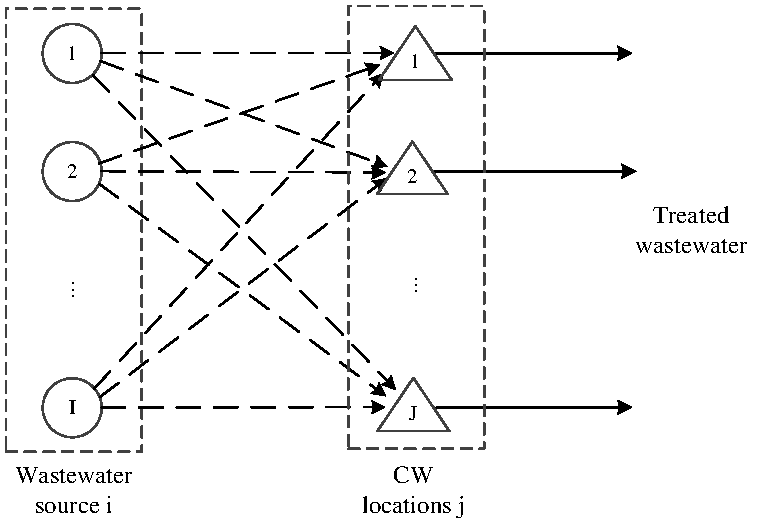
\includegraphics[width=0.7\textwidth]{CWnetwork.pdf}
	\caption{Superstructure of a decentralized CW treatment system network}
	\label{fig:network}
\end{figure}

In general, a decentralized constructed wetlands system in a region can be represented as in Fig. \ref{fig:network}. Wastewater is generated from the sources $I$ and routed to constructed wetlands, where it is treated and discharged or reused on site. Thus, given a set of wastewater sources $I$ and a set of potential constructed wetlands locations $J$, the ultimate objective is to determine how to link the sources to the constructed wetlands, where the wetlands should be located and the size of the wetlands at the site. 

Besides this, in line with regulatory standards for treated water effluent, treatment targets are imposed on a set of pollutants $M$. This means that treated water leaving the constructed wetlands must have pollutant concentrations below specified levels. Depending on the intended use for treated water, treatment targets may be adjusted accordingly for each constructed wetlands site. This constraint directly affects the size of the constructed wetlands for a site as the size of the site determines the pollutant removal rate. It also indirectly affects the routing of the wastewater sources to the treatment sites. 

Thus, a solution is deemed feasible only when it satisfies all the constraints. However, due to natural variation in the environment and pollutant concentration of the influent wastewater, constructed wetlands may not always effectively remove pollutants. In reality, it is also unlikely that the treated wastewater meets the targets all the time. 

Additionally, cost is a major factor for decision makers to take into account hence the best feasible solution should be one that incurs the least cost. The cost consideration affects how the wastewater sources are routed to the treatment sites as the longer the distance, the higher the cost of constructing the pipe to link the source and site up. For the model, the following assumptions are made:

\begin{itemize}
	\setlength{\itemsep}{0pt}
	\setlength{\parskip}{0pt}
	\setlength{\parsep}{0pt}
	\item[-] wastewater from each source $i=1,...,I$ can be allocated to multiple constructed wetlands sites and each constructed wetlands can also treat wastewater from multiple wastewater sources. Sewer lines are needed to be constructed between wastewater sources and constructed wetlands. 
	\item[-] for any location $j=1,...,J$, if it is determined to construct a constructed wetlands, $K$ design options $k=1,...,K$ could be selected. Otherwise, we use $k=0$ to indicate that this location is not chosen to construct any constructed wetlands. 
	\item[-] a list of $M$ pollutants $m=1,...,M$ are evaluated. Treatment target $\tau_j^m$ is set for each pollutant $m$ and each potential site $j$.
\end{itemize}

A basic list of model parameters and decision variables is provided in Table \ref{table:modelparameter}. Other notations would be introduced and defined as per required in the rest of the paper. 

\begin{table}[!htpb]
	\setlength{\extrarowheight}{1.5mm}
	\caption{Notations of model parameters and decision variables}
	\begin{tabular}{|p{1.5cm} p{16cm}|}
		\hline
		\multicolumn{2}{|c|}{Indices} \\
		\hline
		$i$ & index of wastewater sources, $i\in\{1,2,...,I\}$\\
		$j$ & index of potential CW locations, $j\in\{1,2,...,J\}$ \\
		$m$ & index of evaluated water pollutants, $m\in\{1,2,...,M\}$\\
		$k$ & index of CW construction options, $k\in\{0,1,2,...,K\}$\\
		\hline
		\multicolumn{2}{|c|}{Model parameters} \\
		\hline
		$\varepsilon_i^m$ & concentration of pollutant $m$ in the wastewater source $i$ (mg/m$^3$)\\
		$\varepsilon_{in,j}^m$ & concentration of pollutant $m$ in the influent of CW site $j$ (mg/m$^3$)\\
		$\varepsilon_{out,j}^m$ & concentration of pollutant $m$ in the effluent of CW site $j$ (mg/m$^3$)\\
		$\tau_{j}^m$ & treatment target for pollutant $m$ in CW site $j$ (mg/m$^3$)\\
		$F_{i}$ & total wastewater flow generated by source $i$ (m$^3$/d)\\
		$Q_{jk}$ &  flow capacity of CW in option $k$ for site $j$ (m$^3$/d)\\
		$A_{jk}$ & area of CW in option $k$ for site $j$ (m$^2$)\\		$c_{cw,jk}$ & construction cost of CW in design option $k$ for site $j$ (\$) \\	
		$d_{ij}$ & distance between wastewater source $i$ and site $j$ (m)\\
		$c_s$ & unit construction cost of sewer lines per distance (\$/m)\\
		\hline
		\multicolumn{2}{|c|}{Decision variables}\\
		\hline	
		$x_{ij}$ & 0 $\leq$ $x$ $\leq$ 1, proportion of wastewater flow assigned from wastewater source $i$ to the CW in site $j$ \\
		$y_{ij}$ & binary variable, $y_{ij}=1$ if sewer lines are constructed from wastewater source $i$ to CW site $j$ and $0$ otherwise\\
		$z_{jk}$ & binary variable, $z_{jk}=1$ if construction option $k$ is chosen for site $j$ and $0$ otherwise. In particular, $z_{j0}$ denotes the choice of not constructing any CWs in site $j$\\
		\hline	
	\end{tabular}

	\label{table:modelparameter}
\end{table}

Before the uncertainty component is addressed, we may come up with a deterministic model to solve the problem first. The objective of the problem is to minimize the total cost of implementing the system in a region. The following constraints formulate the constructed wetlands construction option, wastewater allocation between sources and constructed wetlands, pollutant removal performance, treatment target fulfillment:

\textbf{Constructed wetlands design options:} Let $z_{jk}$ be a binary variable that describes the design option $k$ selected for the constructed wetlands site $j$. In the case where $k=0$, there will be no constructed wetlands on the potential site $j$. Otherwise, any other values for $k$ will correspond to the respective design options available. When $z_{jk} = 1$, it means that there will be a constructed wetlands of type $k$ at site $j$. The different design options result in different construction costs and pollutant removal capacities. To maintain the logic of the problem, only one design option can be selected at each site. Hence, the following constraint is introduced:
\begin{equation*}
	\begin{split}
	&\sum_{k=0}^{K}z_{jk}=1,~~~\forall j\\
	&z_{jk}\in\{0,1\},~~~\forall j,k
	\end{split}
\end{equation*}

\textbf{Wastewater allocation from sources to sites:} Let $y_{ij}$ be a binary variable that describes the interconnection between the wastewater source $i$ and potential contructed wetlands site $j$. When $y_{ij} = 1$, wastewater is allowed to flow from source $i$ to site $j$. Otherwise, $y_{ij} = 0$. To ensure that the wastewater is allocated consistently, the total of all the flows from a single source $i$ should be equal to the flow generated by source $i$. On top of that, the total volume of wastewater flowing into a constructed wetland cannot exceed the design capacity of the constructed wetland. Finally, there should only be wastewater sent to a site if there is a connection ($y_{ij} = 1$). If $x_{ij}$ represents the proportion of wastewater sent from source $i$ to site $j$, $F_{i}$ is the total wastewater flow from source $i$ and $Q_{jk}$ is the maximum flow capacity accepted by site $j$ with design option $k$:
\begin{alignat*}{2}
    &\sum_{i=1}^{I}x_{ij}F_{i}\leq \sum_{k=0}^{K}Q_{jk}z_{jk},~~ &&\forall j\label{eq:CWcapacity}\\
	&\sum_{j=1}^{J}x_{ij}=1, &&\forall i \nonumber\\
	&0 \leq F_ix_{ij}\leq F_iy_{ij},&&\forall i,j\nonumber\\
	& y_{ij}\in\{0,1\}&&\forall i,j\nonumber
\end{alignat*}
\textbf{Pollutant removal performance and treatment target fulfillment:} First, we consider the influent of the constructed wetlands. The water that is entering the constructed wetlands should have the same amount of pollutants as all of the sources that are contributing wastewater to the site. To determine the pollutant concentration in the effluent, we use a first-order $k-C^*$ model \citep{rousseau2004model} to calculate the pollutant removal. Finally, to ensure that treatment targets are met, the effluent pollutant concentrations should be subject to treatment target constraints. $a_{jk}^m$ is areal rate constant for pollutant treatment. 
\begin{alignat*}{2}
	&{\sum_{i=1}^{I}F_{i}y_{ij}\varepsilon_{i}^{m}} = \varepsilon_{in,j}^{m}{\sum_{i=1}^{I}F_{i}y_{ij}} &&\forall j,m\\
	&[\varepsilon_{in,j}^{m}-{c}_{j}^{m*}]\sum_{k=0}^{K}e^{-\frac{A_{jk}}{Q_{jk}}k_{A}^{m}}z_{jk}+c_{j}^{m*} = \varepsilon_{out,j}^{m} &&\forall j,m\\
	&\varepsilon_{out,j}^{m}\leq \tau_{j}^{m}~~~&&\forall j\\
	&a_{jk}^m = e^{-\frac{A_{jk}}{Q_{jk}}k_{A}^{m}}\\
\end{alignat*}
%The following deterministic model is developed from the above constraints. It is a \emph{Mixed-Integer Linear Programming} (MILP) problem (Model D):
\begin{equation*}\label{modelD}
\begin{aligned}
	\text{Model D}:~~&min \sum_{i=1}^{I}\sum_{j=1}^{J}d_{ij}c_s x_{ij} + \sum_{j=1}^{J}\sum_{k=1}^{K}c_{cw,jk}y_{jk}\\~~
	\mbox{s.t.}~~
	&\sum_{i=1}^{I} (a_{jk}^m \varepsilon_i^m + b_{ij}^m) z_{ij} - M(1 - y_{jk}) \leq \tau_{net,j}^m \sum_{i=1}^I z_{ij}  && \forall j,k,m\\
 	&\sum_{i=1}^{I} z_{ij} \leq \sum_{k=0}^K Q_{jk} y_{jk} && \forall j\\
	&\sum_{j=1}^J z_{ij} = F_i && \forall i\\
	&z_{ij} \leq F_i x_{ij} && \forall i,j\\
	&x_{ij} + y_{j0} \leq 1 && \forall i,j\\
	&\sum_{k=0}^{K}y_{jk} = 1&&\forall j\\
	&x_{ij} \in \{0,1\}&&\forall i,j\\
	&y_{jk} \in \{0,1\}&&\forall j,k\\
	&z_{ij} \geq 0&&\forall i,j\\ 
\end{aligned}
\end{equation*}
\pagebreak
\begin{equation*}\label{modelS}
\begin{aligned}
	\text{Model S}:~~&min \frac{1}{N}\sum_{n=1}^N \gamma^n v^n\\~~
	\mbox{s.t.}~~
	%gamma constraint
	&\varepsilon_{out,j}^{mn} - \tau_j^m + M_1(\gamma^n - 1) \leq 0 && \forall j,m,n\\
	%pollutant treatment constraint (problematic)
	&\sum_{i=1}^{I} (a_{jk}^m \varepsilon_i^{mn} - b_{jk}^m) z_{ij}^n - M_2(1 - y_{jk}) = \varepsilon_{out,j}^{mn} \sum_{i=1}^I z_{ij}^n  && \forall j,k,m,n\\
	%cost constraint
	&\sum_{i=1}^{I}\sum_{j=1}^{J}d_{ij}c_s x_{ij} + \sum_{j=1}^{J}\sum_{k=1}^{K}c_{cw,jk}y_{jk} = v^n && \forall n\\
	%capacity constraint
 	&\sum_{i=1}^{I} z_{ij}^n \leq \sum_{k=0}^K Q_{jk} y_{jk} && \forall j,n\\
	%maximum flow from source
	&\sum_{j=1}^J z_{ij}^n = F_i && \forall i,n\\
	%send water only if connected
	&z_{ij}^n \leq F_i x_{ij} && \forall i,j,n\\
	%enforce no connection if there is no CW constructed
	&x_{ij} + y_{j0} \leq 1 && \forall i,j\\
	%only one design per potential CW site
	&\sum_{k=0}^{K}y_{jk} = 1&&\forall j\\
	%binary constraints
	&x_{ij} \in \{0,1\}&&\forall i,j\\
	&y_{jk} \in \{0,1\}&&\forall j,k\\
	%nonnegative constraint
	&z_{ij}^n \geq 0&&\forall i,j,n\\ 
\end{aligned}
\end{equation*}
\newpage
\subsection{Case study: a decentralized CWs system for municipal wastewater treatment}
\subsubsection{Mobile, Alabama}
With 412,992 people, Mobile County is the second most populated county within the state Alabama in the United States. The population of Mobile County has been steadily increasing \citep{uscb2002census}. As populations grow, several fringe communities are created. To manage the wastewater produced by such communities, the traditional approach is to link these fringe communities up with long length large diameter pipes to transport all the wastewater to a single municipal wastewater treatment plant to be processed and then released into nearby water sources. The Mobile Area Water \& Sewer System (MAWSS) serves approximately 530 square kilometres in Mobile County \citep{mawss2015}, mostly through centralised wastewater treatment facilities. However, annual operations and maintenance costs for such centralised wastewater management systems have been shown to be costlier than decentralised ones, where the wastewater is processed and released within the community \citep{mawss2015}. Thus, implementation of decentralised wastewater management systems such as constructed wetlands are being considered to manage costs in the long term. 

\subsubsection{Data Collection}
\textbf{Case Study Area:}\begin{figure}[!b]
	\centering
	\includegraphics[width=0.35\textwidth]{blocks.png}
	\caption{Case study area in Mobile, Alabama.}
	\label{fig:blocks}
\end{figure}
The site chosen for the case study is near Mobile Regional Airport. It is a suburban area, mostly consisting of residences. As the objective of the project is to show how the optimization model can be applied, we have chosen a smaller area to keep the computation resources required reasonable. Hence, the site has been divided into 14 blocks based on six census tract blocks. The blocks are represented with blue outlines in Fig. \ref{fig:blocks}. Geographic information about the region listed in Table \ref{table:geodata} was also retrieved from the census. \citep{acs2015} For each block, we have assumed a point source for the wastewater (see red circles).

Potential sites for the constructed wetlands were identified from Google Maps and represented in Fig. \ref{fig:blocks} as green rectangles. These areas are empty and thus the construction of wetlands there will impact few residents negatively. A point location is used to represent each of these sites. The coordinates of the potential sites are stated in Table \ref{table:cwdata}. The distances between the wastewater sources and potential sites were calculated as well and stated in Table \ref{table:distdata}. 

\textbf{Pollutants:} Once again, to keep the model manageable, we have narrowed down the number of pollutants to three, as seen in Table \ref{table:polldata}. The pollutants have been selected based on the effects of pollution if these substances were not removed. In this case study, we will set the treatment target to be the same regardless of the intended use for the treated water.

\textbf{Design options:} We have determined four design options for the constructed wetlands and their respective construction costs can be found in Table \ref{table:ccwdata}. The formula for estimating the cost can be found in \cite{kadlec2009}.

\textbf{Sewer pipe construction cost:} Based on \cite{kadlec2009}, the normal size of sewer pipes for treatment wetlands vary from $10-30 cm$ diameter pipes. Hence, the sewer pipe construction cost is estimated to be about $US\$134/m$ \citep{usepa2000} after revising to latest prices. \\

The above information provides a good set-up to determine optimal locations for constructed wetlands to be built within Mobile, Alabama. 

\section{Further Directions}
Proceeding from here, the next step would be to find a solution for the deterministic model, which will be done using MATLAB. After which, work will commence on developing the probabilistic model and running it. 


%\section{Conclusions}
\newpage
\section*{Appendix}\label{Chap:appendix}

\begin{table}[!h]
	\caption{Geographical information about the 14 blocks.}
	\label{table:geodata}
	\centering
	\begin{tabular}{c c c c c c}
		\csvautotabular{data/blockgeo.csv}
	\end{tabular}
\end{table}

\begin{table}[!h]
	\caption{Coordinates of the potential constructed wetlands sites.}
	\label{table:cwdata}
	\centering
	\begin{tabular}{ c c c }
		\csvautotabular{data/cwgeo.csv}
	\end{tabular}
\end{table}

\begin{table}[!h]
	\caption{Distance in $km$ between the wastewater sources and potential constructed wetlands sites.}
	\label{table:distdata}
	\centering
	\begin{tabular}{ c c c c c c c c c c c c}
		\csvautotabular{data/dist.csv}
	\end{tabular}
\end{table}

\begin{table}[!h]
	\caption{Selected pollutants with the respective indicators coupled with average pollutant concentration in the wastewater source and the treatment targets.}
	\label{table:polldata}
	\centering
	\makebox[\linewidth]{
	\begin{tabular}{c c c c c}
		\csvautotabular{data/pollutants.csv}
	\end{tabular}
	}
\end{table}

\begin{table}[!h]
	\caption{Construction cost of constructed wetlands with four different design options as well as projected area and flow capacity.}
	\label{table:ccwdata}
	\centering
	\begin{tabular}{c c c c}
		\csvautotabular{data/ccw.csv}
	\end{tabular}
\end{table}

\addcontentsline{toc}{chapter}{Appendix}
\setcounter{equation}{0}
\renewcommand{\theequation}{A.\arabic{equation}}
\setcounter{figure}{0}
\renewcommand{\thefigure}{A.\arabic{figure}}
\setcounter{section}{0}
\renewcommand{\thesection}{A-\arabic{section}}
\newpage

\clearpage
\section*{References}
\bibliographystyle{apalike} 
\bibliography{mobile}

\end{document}

